\RequirePackage{fix-cm}
\documentclass[titlepage]{article}

\usepackage{fullpage}   % Use the whole page
\usepackage{fancyhdr}   % Nice headers/footers
\usepackage{graphicx}   % Importing graphics
\usepackage{graphics}   % Importing graphics
\usepackage{mdwlist}    % For itemize* and enumerate*
\usepackage{hyperref}   % Hyperlink references and URLs
\usepackage{subfig}
\usepackage{appendix}
\usepackage{listings}
%\usepackage{todonotes}
\usepackage[usenames,dvipsnames]{xcolor}	% Logo
\usepackage{tikz,ifthen}			% Logo
\usepackage{pgf}				% Logo
\usepackage{scalefnt}				% Logo
\usepgfmodule{shapes}				% Logo
\usepgfmodule{plot}				% Logo
\usetikzlibrary{shapes,snakes,arrows,decorations}

\hypersetup{
    colorlinks=true,
    linkcolor=blue,
    urlcolor=blue,
    pdftitle={AHOY Software Requirements Specification V6},
    pdfauthor={Dustin Ingram, Aaron Rosenfeld, Maria Kolakowska, Frank Clark}
}

% So we can number paragraphs too
\setcounter{secnumdepth}{5}

% For headers and footers
\setlength{\headheight}{15pt}
\setlength{\headsep}{25pt}
\pagestyle{fancy}
	
% Page style for the title page
\fancypagestyle{plain}{
    \fancyhf{}
    \renewcommand{\headrulewidth}{0pt}
    \renewcommand{\footrulewidth}{0pt}
}

% Just so we don't have to specify this twice
\newcommand\mytitle{Software Requirements Specification}
\newcommand\mydate{\today}

% Page style for every other page
\fancyhf{} % clear all header and footer fields
\fancyhead[L]{AHOY}
\fancyhead[C]{\mytitle}
\fancyhead[R]{\mydate}
\fancyfoot[C]{\thepage}
\renewcommand{\headrulewidth}{0.4pt}
\renewcommand{\footrulewidth}{0.4pt}

\title{\textbf{\mytitle}}
\author{
	Frank Clark \\\url{francis.j.clark@drexel.edu}
    \and Dustin Ingram \\\url{dustin.s.ingram@drexel.edu}
	\and Maria Kolakowska \\\url{maria.j.kolakowska@drexel.edu}
    \and Aaron Rosenfeld \\\url{aaron.rosenfeld@drexel.edu}
}
\date{\mydate\\Version 6}

\begin{document}
\pagenumbering{roman}

\begin{figure}
   % \vspace{-2em}
    \centering
    \scalebox{0.8}{

\begin{tikzpicture}[scale=1]
	
	\pgfsetlinewidth{3pt}

	% Background
	\color{cyan!70!black}
	\pgfpathmoveto{\pgfpointxy{-5}{2}}
	\pgfpathlineto{\pgfpointxy{-5}{11}}
	\pgfpathlineto{\pgfpointxy{-2}{11.9}}	
	\pgfpathlineto{\pgfpointxy{2}{11.9}}	
	\pgfpathlineto{\pgfpointxy{5}{11}}
	\pgfpathlineto{\pgfpointxy{5}{2}}
	\pgfpathclose 
	\pgfusepath{fill,stroke} 

	% Base
	\color{green!70!black}
	\pgfsetstrokecolor{black}
	\pgfpathmoveto{\pgfpointxy{-2}{1.5}}
	\pgfpathcurveto{\pgfpointxy{-2}{1.5}}{\pgfpointxy{-6}{1.5}}{\pgfpointxy{-6}{2.5}}
	\pgfpathlineto{\pgfpointxy{-6}{4}}
	\pgfpathlineto{\pgfpointxy{6}{4}}
	\pgfpathlineto{\pgfpointxy{6}{2.5}}
	\pgfpathcurveto{\pgfpointxy{6}{1.5}}{\pgfpointxy{2}{1.5}}{\pgfpointxy{2}{1.5}}
	\pgfpathclose 
	\pgfusepath{fill,stroke} 

	% Curtains
	\color{red!70!black}
	\pgfsetstrokecolor{black}

	% Left
	\pgfpathmoveto{\pgfpointxy{-6}{11}}
	\pgfpathlineto{\pgfpointxy{-6}{2.5}}
	\pgfpathcurveto{\pgfpointxy{-6}{2.2}}{\pgfpointxy{-3.5}{2.2}}{\pgfpointxy{-3.5}{2.5}}
	\pgfpathcurveto{\pgfpointxy{-3.5}{3}}{\pgfpointxy{-3.5}{4}}{\pgfpointxy{-4.5}{5}}
	\pgfpathcurveto{\pgfpointxy{-2.5}{7}}{\pgfpointxy{-4}{11}}{\pgfpointxy{-3}{11.5}}
	\pgfpathcurveto{\pgfpointxy{-4}{11}}{\pgfpointxy{-2.5}{7}}{\pgfpointxy{-4.5}{5}}
	\pgfpathcurveto{\pgfpointxy{-2.5}{7}}{\pgfpointxy{-6}{11}}{\pgfpointxy{-3}{11.5}}
	\pgfpathcurveto{\pgfpointxy{-6}{11}}{\pgfpointxy{-2.5}{7}}{\pgfpointxy{-4.5}{5}}
	\pgfpathcurveto{\pgfpointxy{-2.5}{7}}{\pgfpointxy{-8}{11}}{\pgfpointxy{-3}{11.5}}
	\pgfpathcurveto{\pgfpointxy{-8}{11}}{\pgfpointxy{-2.5}{7}}{\pgfpointxy{-4.5}{5}}
	\pgfpathcurveto{\pgfpointxy{-2.5}{7}}{\pgfpointxy{-2.5}{11}}{\pgfpointxy{-3}{11.5}}
	\pgfusepath{fill,stroke}

	% Right
	\pgfsetlinewidth{3pt}
	\pgfpathmoveto{\pgfpointxy{6}{11}}
	\pgfpathlineto{\pgfpointxy{6}{2.5}}
	\pgfpathcurveto{\pgfpointxy{6}{2.2}}{\pgfpointxy{3.5}{2.2}}{\pgfpointxy{3.5}{2.5}}
	\pgfpathcurveto{\pgfpointxy{3.5}{3}}{\pgfpointxy{3.5}{4}}{\pgfpointxy{4.5}{5}}
	\pgfpathcurveto{\pgfpointxy{2.5}{7}}{\pgfpointxy{4}{11}}{\pgfpointxy{3}{11.5}}
	\pgfpathcurveto{\pgfpointxy{4}{11}}{\pgfpointxy{2.5}{7}}{\pgfpointxy{4.5}{5}}
	\pgfpathcurveto{\pgfpointxy{2.5}{7}}{\pgfpointxy{6}{11}}{\pgfpointxy{3}{11.5}}
	\pgfpathcurveto{\pgfpointxy{6}{11}}{\pgfpointxy{2.5}{7}}{\pgfpointxy{4.5}{5}}
	\pgfpathcurveto{\pgfpointxy{2.5}{7}}{\pgfpointxy{8}{11}}{\pgfpointxy{3}{11.5}}
	\pgfpathcurveto{\pgfpointxy{8}{11}}{\pgfpointxy{2.5}{7}}{\pgfpointxy{4.5}{5}}
	\pgfpathcurveto{\pgfpointxy{2.5}{7}}{\pgfpointxy{2.5}{11}}{\pgfpointxy{3}{11.5}}
	\pgfusepath{fill,stroke}

	% Top
	%     Top-left
	\pgfpathmoveto{\pgfpointxy{-2}{12}}
	\pgfpathcurveto{\pgfpointxy{-2}{12}}{\pgfpointxy{-6}{12}}{\pgfpointxy{-6}{11}}
	\pgfpathcurveto{\pgfpointxy{-5}{9}}{\pgfpointxy{-2}{11}}{\pgfpointxy{-2}{11.85}}
	\pgfpathcurveto{\pgfpointxy{-2}{11.5}}{\pgfpointxy{-4.5}{9.5}}{\pgfpointxy{-6}{11}}
	\pgfpathcurveto{\pgfpointxy{-4.5}{9.5}}{\pgfpointxy{-2}{11.5}}{\pgfpointxy{-2}{11.85}}
	\pgfpathcurveto{\pgfpointxy{-2}{12}}{\pgfpointxy{-3.5}{10.4}}{\pgfpointxy{-6}{11}}
	\pgfpathcurveto{\pgfpointxy{-3.5}{10.4}}{\pgfpointxy{-2}{12}}{\pgfpointxy{-2}{11.85}}

	%    Top-middle
	\pgfpathcurveto{\pgfpointxy{-1}{10.5}}{\pgfpointxy{1}{10.5}}{\pgfpointxy{2}{11.85}}
	\pgfpathcurveto{\pgfpointxy{1}{10.5}}{\pgfpointxy{-1}{10.5}}{\pgfpointxy{-2}{11.85}}	
	\pgfpathcurveto{\pgfpointxy{-1}{11}}{\pgfpointxy{1}{11}}{\pgfpointxy{2}{11.85}}
	\pgfpathcurveto{\pgfpointxy{1}{11}}{\pgfpointxy{-1}{11}}{\pgfpointxy{-2}{11.85}}	
	\pgfpathcurveto{\pgfpointxy{-1}{10}}{\pgfpointxy{1}{10}}{\pgfpointxy{2}{11.85}}

	%    Top-right
	\pgfpathcurveto{\pgfpointxy{2}{11.5}}{\pgfpointxy{4.5}{9.5}}{\pgfpointxy{6}{11}}
	\pgfpathcurveto{\pgfpointxy{4.5}{9.5}}{\pgfpointxy{2}{11.5}}{\pgfpointxy{2}{11.85}}
	\pgfpathcurveto{\pgfpointxy{2}{12}}{\pgfpointxy{3.5}{10.4}}{\pgfpointxy{6}{11}}
	\pgfpathcurveto{\pgfpointxy{3.5}{10.4}}{\pgfpointxy{2}{12}}{\pgfpointxy{2}{11.85}}
	\pgfpathcurveto{\pgfpointxy{2}{11}}{\pgfpointxy{5}{9}}{\pgfpointxy{6}{11}}
	\pgfpathcurveto{\pgfpointxy{6}{12}}{\pgfpointxy{2}{12}}{\pgfpointxy{2}{12}}
	\pgfpathclose 
	\pgfusepath{fill,stroke} 

	% Rope
	%     Rope-right
	\pgfsetstrokecolor{black}
	\pgfpathmoveto{\pgfpointxy{-4.5}{5}}
	\pgfpathcurveto{\pgfpointxy{-4.5}{5}}{\pgfpointxy{-6}{5}}{\pgfpointxy{-6}{5.5}}
	\pgfusepath{stroke}	
	%     Rope-left
	\pgfsetstrokecolor{black}
	\pgfpathmoveto{\pgfpointxy{4.5}{5}}
	\pgfpathcurveto{\pgfpointxy{4.5}{5}}{\pgfpointxy{6}{5}}{\pgfpointxy{6}{5.5}}
	\pgfusepath{stroke}

	\node[color=black] at (0,0) {{\scalefont{10.0}STAGE}};

	%% Just kinda a pretty path...
	%% \pgfpathmoveto{\pgfpointxy{-2}{1.5}}
	%% \pgfpathcurveto{\pgfpointxy{-2}{1.5}}{\pgfpointxy{-6}{1.5}}{\pgfpointxy{-6}{2.5}}
	%% \pgfpathcurveto{\pgfpointxy{-5}{4.5}}{\pgfpointxy{-2}{2.5}}{\pgfpointxy{-2}{3.35}}
	%% \pgfpathcurveto{\pgfpointxy{-1}{3.5}}{\pgfpointxy{1}{3.5}}{\pgfpointxy{2}{3.35}}
	%% \pgfpathcurveto{\pgfpointxy{2}{2.5}}{\pgfpointxy{5}{4.5}}{\pgfpointxy{6}{2.5}}
	%% \pgfpathcurveto{\pgfpointxy{6}{1.5}}{\pgfpointxy{2}{1.5}}{\pgfpointxy{2}{1.5}}
	%% \pgfpathclose 
\end{tikzpicture}
}
    \vspace{-4em}
\end{figure}

\maketitle

\begin{abstract}
AHOY is an event-based simulation environment used to compare the effectiveness of different combinations of software agents, network configurations, and sensor data in real-world environments.  It is comprised of a distributed simulation engine, visualizer, and programming interface through which developers create agent software and network topologies.  Communication between virtual nodes is also simulated, providing highly realistic scenarios.
\end{abstract}

\setcounter{tocdepth}{4}
\tableofcontents
\pagebreak
\listoffigures
\pagebreak
\pagenumbering{arabic}

%\listoftodos

%___________________________________________________________________________

\section{Introduction%
  \label{introduction}%
}

%___________________________________________________________________________

\subsection{Purpose%
  \label{purpose}%
}

This requirements document defines the functional and non-functional requirements for the AHOY project.  These requirements include, but are not limited to, the performance, interfaces, and hardware goals and limitations.  The information presented here is intended for the development team and the external stakeholders, currently Dr. William Regli, Mr. Joseph B. Kopena, Mr. Joeseph P. Macker, and The U.S. Naval Research Laboratory.

%___________________________________________________________________________

\subsection{Scope%
  \label{scope}%
}
The goal of the AHOY project is to provide a system for testing multiple agents across varying scenarios and topologies, in a distributed, event-driven way. AHOY gives the user the ability to quantitatively examine the effectiveness of specific agent designs as well as a focus on additional factors relevant to the network, including network connectivity, connection fidelity, and the agent's ability to process and transmit data.

AHOY consists of six main components: a simulation, a networking engine, an event channel, world entities, agents, and sensors.  The simulation orchestrates initialization and termination of an experiment.  The networking engine handles all inter-entity communications based on real-world network models.  The event channel is the means by which all events are disseminated to distributed simulation nodes.  World entities are any physical object within the simulation (e.g. nodes).  Agents are software which runs on nodes, and may interact with local sensors which sense the simulated environment.

Users of AHOY are researchers looking to improve or test their current agent/network interactions across different topology and scenario combinations.  
%___________________________________________________________________________

\subsection{Definitions, Acronyms, and Abbreviations%
  \label{definitions}%
}

\begin{description}
\item[Agent]
	Agents are simulated pieces of software that run on nodes in the simulation. An agent is described by a set of precondition-trigger-action tuples.  When the trigger (an event) occurs, if and only if the precondition is satisfied, the action will be invoked.

\item[Distribution]
	Distribution refers to the process of distributing the simulation across a multi-platform physical cluster.  This allows the system to exceed the number of nodes per platform for a single simulation at the system's discretion.  A framework will be provided to allow the user to distribute their simulation. 	

\item[Node]
	Nodes are virtual or physical machines that consist of agents and network interfaces.  If nodes are virtual, many nodes may run on one physical machine.  

\item[Scenario]
	Scenario is comprised of a scripted language indicating the location simulated nodes within the virtual world. These nodes consist of agents (see definition of `Agent') and non-agent world objects such as planes, boats, ground vehicles, etc. 

\item[Terrain]
	Terrain refers to the simulated landscape.  This includes attributes such as elevation, buildings, and the locations of water. 

\item[Topology]
	Topology describes the possibly time-dependant connections between nodes and their characteristics (e.g. aradio model).
    
\end{description}

%___________________________________________________________________________

\subsection{References%
  \label{references}%
}

These documents have been used as reference materials for various technologies involved with this project.
%
\begin{itemize*}
	\item SPEYES: Sensing and Patrolling Enablers Yielding Effective SASO: \url{http://ieeexplore.ieee.org/xpls/abs_all.jsp?arnumber=1559616}
	\item Service Sniffer Requirements Document: \url{http://servicesniffer.net/documents/requirements.html}
    \item Developing an Agent Systems Reference Architecture: \url{www.cs.drexel.edu/~dn53/papers/paper_cameraready.pdf}
\end{itemize*}


%___________________________________________________________________________

\subsection{Overview%
  \label{overview}%
}

The rest of this document is organized as follows: 
\begin{itemize*}
	\item[-]Section \ref{overall-description} gives a high level overview of the project requirements.  
	\item[-]Section \ref{specific-requirements} gives more detailed project requirements.  
	\item[-]Sections \ref{input-formats} and \ref{output-formats} provides detail in the inputs and outputs of the system, 
	\item[-]Section \ref{functional} specifies what the software will do, 
\end{itemize*}
The rest of Section \ref{specific-requirements} explains other minor requirements.

%___________________________________________________________________________

\section{Overall Description%
  \label{overall-description}%
}

%___________________________________________________________________________

\subsection{Product Perspective%
  \label{product-perspective}%
}

AHOY is a software testbed for comparing combinations of sensors, agents, and networks.  It allows users to quickly set up a scenario and interchange these components, something not possible in the real-world.

%___________________________________________________________________________

\subsubsection{System Interfaces%
  \label{system-interfaces}%
}

AHOY combines:
\begin{itemize}
    \item \textbf{Scenario Definition}: Defines a scenario including locations of world entities, agents, sensors, and network configurations
    \item \textbf{Agent Framework}: Allows for the creation of intelligent agents
    \item \textbf{Distribution Framework}: Distributes a simulation across multiple physical computers
\end{itemize}

%___________________________________________________________________________

\subsubsection{User Interfaces%
  \label{user-interfaces}%
}

AHOY is intentionally designed to provide no specific user interface in the traditional sense. Instead, it provides an extensive and comprehensive API, for creating a simulation, interacting with an experiment as it is running, monitoring events from a global viewpoint, and recording the results of an experiment for analysis. This ultimately offers flexibility for the end user, as separate, pre-existing user interfaces can be modified to support AHOY's software API, or simply be created from scratch to explicitly satisfy the user's needs. 

\subsection{Product Functions%
  \label{product-functions}%
}

This software is a testbed, where the users specify an environment, network configuration, and agent software running in the simulation. Each of these items may be varied independently at runtime.

The primary function of this software is to coordinate an event-based simulation comprised of virtual nodes, other world objects, agent software, and network devices.  Specifically the software starts simulations, handles all events, and determines when a scenario is complete.

Simulation of inter-node communications is handled by AHOY's networking component.  This component provides realistic simulation of network links and virtual node networking stacks.

%___________________________________________________________________________


\subsection{User Characteristics%
  \label{user-characteristics}%
}

The system has four different types of users.  Each type of user has different goals and needs to use different parts of the system.  These user roles, while they may be performed by the same user, are here split into the four distinct roles for clarity:

%___________________________________________________________________________

\subsubsection{Fictional User: Alice, Project Manager%
  \label{alice}%
}

Alice uses AHOY for demonstrations and to acquire funding for research.  Alice wants to complete the tasks below with an existing visualization:

\begin{itemize*}
    \item Start a simulation
    \item View the simulation in real time
    \item Visualize simulation events including link changes and entity movements
    \item View output from agents if implemented
\end{itemize*}

\begin{figure}
    \centering
    \begin{tikzpicture} [scale=.4]
    \path[fill=yellow!10,rounded corners, draw=black!50, dashed]
                (-3,10) rectangle (10,-3);
    \draw (-3,10) node[anchor=north west, draw=none]{1.};
    
    \draw[very thick,dashed] (0,0) circle (2.2);
    \draw[very thick,dashed] (3,2) circle (2.2);
    \draw[very thick,dashed] (7,7) circle (2.2);
    \draw[very thick,dashed] (6,1) circle (2.2);
    \draw[very thick,dashed] (1,6) circle (2.2);
    
    \node[diamond, draw, fill=green!20] (a) at (0,0) {A};
    \node[diamond, draw, fill=green!20] (b) at (3,2) {B};
    \node[diamond, draw, fill=green!20] (c) at (7,7) {C};
    \node[diamond, draw, fill=green!20] (d) at (6,1) {D};
    \node[diamond, draw, fill=green!20] (e) at (1,6) {E};
    
    %%two
    \path[fill=yellow!30,rounded corners, draw=black!50, dashed]
                (10,10) rectangle (23,-3);
    \draw (10,10) node[anchor=north west, draw=none]{2.};
    
    \draw[very thick,dashed] (14,2) circle (2.2);
    \draw[very thick,dashed] (16,4) circle (2.2);
    \draw[very thick,dashed] (20,7) circle (2.2);
    \draw[very thick,dashed] (19,1) circle (2.2);
    \draw[very thick,dashed] (14,6) circle (2.2);
    
    \node[diamond, draw, fill=red!20] (a2) at (14,2) {A};
    \node[diamond, draw, fill=red!20] (b2) at (16,4) {B};
    \node[diamond, draw, fill=green!20] (c2) at (20,7) {C};
    \node[diamond, draw, fill=green!20] (d2) at (19,1) {D};
    \node[diamond, draw, fill=red!20] (e2) at (14,6) {E};
    
    \path[-, very thick] (b2) edge (a2);
    \path[-, very thick] (b2) edge (e2);
   
    %%three
    \path[fill=yellow!50,rounded corners, draw=black!50, dashed]
                (23,10) rectangle (36,-3);
    \draw (23,10) node[anchor=north west, draw=none]{3.};

    \draw[very thick,dashed] (27,2) circle (2.2);
    \draw[very thick,dashed] (29,4) circle (2.2);
    \draw[very thick,dashed] (33,4) circle (2.2);
    \draw[very thick,dashed] (31,2) circle (2.2);
    \draw[very thick,dashed] (27,6) circle (2.2);
    
    \node[diamond, draw, fill=red!20] (a3) at (27,2) {A};
    \node[diamond, draw, fill=red!20] (b3) at (29,4) {B};
    \node[diamond, draw, fill=red!20] (c3) at (33,4) {C};
    \node[diamond, draw, fill=red!20] (d3) at (31,2) {D};
    \node[diamond, draw, fill=red!20] (e3) at (27,6) {E};
    
    \path[-, very thick] (b3) edge (a3);
    \path[-, very thick] (b3) edge (e3);
    \path[-, very thick] (b3) edge (d3);
    \path[-, very thick] (d3) edge (c3);
   
    %\begin{scope}[very thick,dashed]
    %\draw (0,0) circle (.5cm);
    %\draw (0,0) circle (1cm);
    %\end{scope} \draw[thin] (0,0) circle (1.5cm);
 \end{tikzpicture}

    \caption[Prototype Use Case Diagram]%
    {A prototype of what ``Bob'' may create: \emph{1.} Agents have been configured to perform random walks within a boundary, and each contains a wireless interface. \emph{2.} When nodes recieve an event indicating they are in range of another node, they hold their position and create a network link. \emph{3.} A static network is formed.}   
\end{figure}

\subsubsection{Fictional User: Bob, Agent Algorithm Researcher%
  \label{bob}%
}

Bob researches agent algorithms and uses AHOY to compare their effectiveness.  Bob wants to complete the tasks below:

\begin{itemize*}
    \item Use the API to implement agents which run on network nodes
    \item Use a visualizer to assure scenarios are properly setup
    \item Run scenarios many times, without a visualization
    \item Collect aggregate data from scenario trials via the API
\end{itemize*}

\subsubsection{Fictional User: Carol, Network Protocol Developer%
  \label{bob}%
}

Carol uses AHOY to test networking protocols.  Specifically, she tries different network protocols with a single agent setup to find the best combination.  Carol wants to complete the tasks below:

\begin{itemize*}
    \item Use the networking component to implement networking protocols
    \item Run scenarios many times
    \item Collect aggregate data from scenario trials via the API
\end{itemize*}

\subsubsection{Fictional User: Dave, Large Scale Simulator%
  \label{bob}%
}

Dave uses AHOY to run large scale simulations which run slower than real-time on his personal computer.  Dave wants to complete the tasks below:

\begin{itemize*}
    \item Distribute agent instances to multiple physical machines
    \item Abstract the physical links from the simulation
    \item Coordinate data collection after simulations
\end{itemize*}
%___________________________________________________________________________

\subsection{Constraints%
  \label{constraints}%
}

No piece of this system requires elevated privileges.  The physical machines running the simulation must have at least one network interface.

%___________________________________________________________________________

\subsection{Assumptions and Dependencies%
  \label{assumptions-and-dependencies}%
}

It is assumed that a user, administrator, or developer has the ability to install Python version 2.6.0 or higher.  No additional libraries are required.

%___________________________________________________________________________

\section{Specific Requirements%
  \label{specific-requirements}%
}

\subsection{Functional Requirements%
    \label{functional}%
}

\subsubsection{Simulation Engine}
	The following applies to AHOY's Simulation Engine:
    \paragraph{Timing} The Simulation Engine runs in real-time.
    \paragraph{Maximum Models} The Simulation Engine keeps in memory up to 500 nodes.
    \paragraph{Startup} The Simulation Engine interprets the scenario definition and distributes world entities to distributed nodes.
    \paragraph{Shutdown} The Simulation Engine responds to any shutdown requests from the user and terminates the simulation.

\subsubsection{Scenario Definition}
	\paragraph{Location} The Scenario Definition defines existence and location of all world entities.
    \paragraph{Agents} The Scenario Definition defines the agents which run on each virtual node.
    \paragraph{Sensors} The Scenario Definition defines the sensors which run on each virtual entity.
	\paragraph{Networks} The Scenario Definition specifies networks to which interfaces may connect.  Networks are described with a unique identifier and physical layer model (e.g. 802.11, Ethernet).
	\paragraph{Interfaces} The Scenario Definition specifies the interfaces on each virtual node and on which network they are connected.

\subsubsection{Distribution Framework}
	\paragraph{Physical Distribution} The Distribution Framework distributes virtual entities evenly across physical nodes. Further, it handles the establishment and initialization of entities, sensors, and agents on their respective physical entity.
	\paragraph{Simulation Server} The Distribution Framework organizes physical nodes to interact with the simulation server.

%___________________________________________________________________________

\subsubsection{Data Storage%
  \label{data-storage}%
}
    \paragraph{Outside Databases} No outside database system is used for data storage, unless it is introduced by the user via the API.
    \paragraph{Scenario Definitions} Scenario definitions are stored as Python files.

%___________________________________________________________________________

\subsection{Non-Functional Requirements} 
%___________________________________________________________________________

\subsubsection{Hardware Interfaces%
  \label{hardware-interfaces}%
}

AHOY requires that the machine running the system has at least one network interface for distribution.  If distribution is not desirable, only a loopback (\texttt{lo}) interface is necessary.
%___________________________________________________________________________

\subsubsection{Software Interfaces%
  \label{software-interfaces}%
}

AHOY relies on the installation of Python version 2.6.0 or higher.  Python version 3.0 and higher is not supported.

%___________________________________________________________________________

\subsubsection{Memory Constraints%
  \label{memory-constraints}%
}

AHOY requires all distributed machines to have at least 4GB of RAM.

%___________________________________________________________________________

\subsubsection{Site Adaptation Requirements%
  \label{site-adaptation-requirements}%
}

AHOY requires that the system is configured per-site to create a distributed simulation, or to interact on-the-fly.

%__________________________________________________________________________

\subsubsection{Operating System%
  \label{operating-system}%
}

AHOY is able to run on Unix, Linux, and Mac

%__________________________________________________________________________

\subsubsection{Processor% 
  \label{processor}%
}

AHOY requires at least a 32- or 64-bit x86 3.0 GHz processor

%__________________________________________________________________________

\subsection{Input Formats%
  \label{input-formats}%
}

The AHOY input format is a single Python script for each scenario.  No additional input formats are used.

%___________________________________________________________________________

\subsection{Output Formats%
  \label{output-formats}%
}

AHOY does not natively output data to files.  Users may subscribe to the event channel via the API to record any information necessary.

%___________________________________________________________________________
\subsection{Extensibility%
  \label{extensibility}%
}
\subsubsection{Customization}
    \paragraph{Custom Scenarios} The system provides a means for users to create custom scenarios
    \paragraph{Custom Agents} The system provides a means for users to create custom agents.
    \paragraph{Custom Networks} The system provides a means for users to create custom network models.
    \paragraph{Custom Sensors} The system provides a means for users to create custom sensors.

\subsection{Testing%
    \label{testing}%
}
All code with in the system must be tested. Core functionality of the software has 100\% code coverage with automated unit and integration tests.  Unit tests cover the algorithms used in our system while integration tests are used to test our data-flow.  

\section{System Evolution}

With more time, the AHOY team could create additional tools to aid in the development of more complex agents, so that user customization does not become too granular.  Furthermore, tools which can automate or assist in data collection and parsing could be implemented.  Even further development could lead to a platform that included Windows or other operating systems.

%___________________________________________________________________________

\subsection{Documentation%
  \label{documentation}%
}
\begin{enumerate}
    \item The software provides a User Manual containing step-by-step instructions for user perspective in Section~\ref{user-characteristics}.
    \item The software provides Developer Documentation containing:
    \begin{enumerate}
        \item Scenario Definition usage
        \item Information regarding creating custom agents, sensors, and network models
    \end{enumerate}
\end{enumerate}

%___________________________________________________________________________

\appendix
\pagebreak

\end{document}
